\documentclass{beamer}
\usepackage{beamerthemesplit}
\usetheme{innoQ}
\setbeamertemplate{navigation symbols}{}
% \beamersetuncovermixins{\opaqueness<1>{15}}{\opaqueness<2->{10}}
\def\pdfshellescape{1}
\usetikzlibrary{calc}
% \usepackage[utf8]{inputenc}
\usepackage[T1]{fontenc}
\usepackage{textcomp}
% \usepackage{listings}
\usepackage{minted}
\usepackage{graphicx}
\usepackage{wasysym}
\usepackage{url}        % for displaying URLs correctly
\usepackage{soul}       % for \caps
% \usepackage{ulem}       % for \sout
\usepackage{hyperref}
\usepackage[ngerman]{babel}
\usepackage{pifont}

\date{Booster 2013, Bergen, NO \\ 2013-03-14}
\author{FND \& wvk, innoQ Deutschland GmbH}

\title{ROCA}
\subtitle{Embrace the Web}

\definecolor{links}{HTML}{2A1B81}
\hypersetup{colorlinks,linkcolor=,urlcolor=links}

% fonts
\RequirePackage{fontspec}
\defaultfontfeatures{Mapping=tex-text}
\setmainfont[BoldFont={MetaOT-Medi}, BoldItalicFont={MetaOT-MediIta}, ItalicFont={MetaOT-NormIta}, SlantedFont={MetaOT-NormIta}, BoldSlantedFont={MetaOT-MediIta}, Ligatures=TeX]{MetaOT-Norm}
\setsansfont[BoldFont={MetaOT-Medi}, BoldItalicFont={MetaOT-MediIta}, ItalicFont={MetaOT-NormIta}, SlantedFont={MetaOT-NormIta}, BoldSlantedFont={MetaOT-MediIta}, Ligatures=TeX]{MetaOT-Norm}
\newfontfamily\metamedifamily[SlantedFont={MetaOT-MediIta}]{MetaOT-Medi}


\newcommand{\rocaok}{\ding{51}}
\newcommand{\rocafail}{\ding{55}}

\begin{document}
  {\usebackgroundtemplate{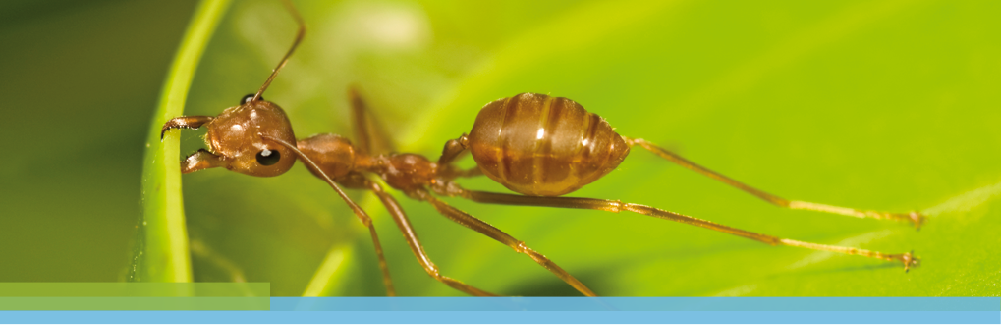
\includegraphics[width=\paperwidth]{images/innoqbg.png}}

  \begin{frame}[plain]
    \titlepage
  \end{frame}
}

\setcounter{tocdepth}{1}

\begin{frame}{Embrace the Web}
  \begin{columns}
    \begin{column}{4.4cm}
      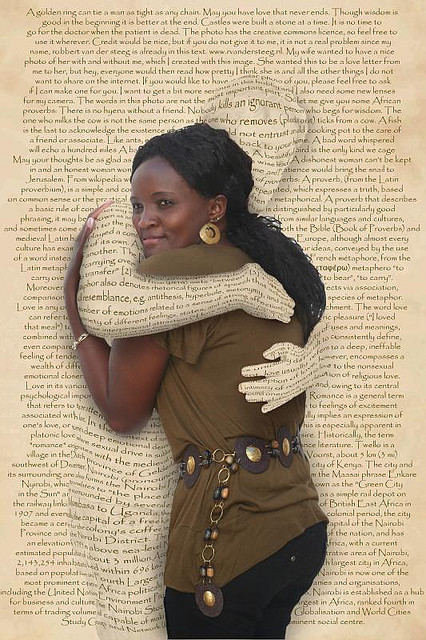
\includegraphics[width=4cm]{images/embrace.jpg}
      \\
      \tiny source: \href{http://www.flickr.com/photos/robbie73/4289385819/}{Robbert van der Steeg}
    \end{column}

    \begin{column}{6.6cm}
      \tableofcontents
    \end{column}
  \end{columns}
\end{frame}

\section{Hej.}

\begin{frame}{\insertsectionhead}
  \begin{itemize}
    \item[FND] \href{mailto:fnd@innoq.com}{Frederik Dohr} \\
        recovering SPA enthusiast (\ensuremath{\rightarrow} TiddlyWiki)
    \item[]
    \item[wvk] \href{mailto:wvk@innoq.com}{Willem van Kerkhof} \\
        practitioner of others' preaches
  \end{itemize}

  %NOTE general introduction: participants' prior experience & expectations
  %NOTE * technologies (languages & frameworks)
  %NOTE * patterns
  %NOTE * common issues
  %NOTE
  %NOTE /!\ interactivity desired

\end{frame}

\section{What's ROCA?}

{
  \usebackgroundtemplate{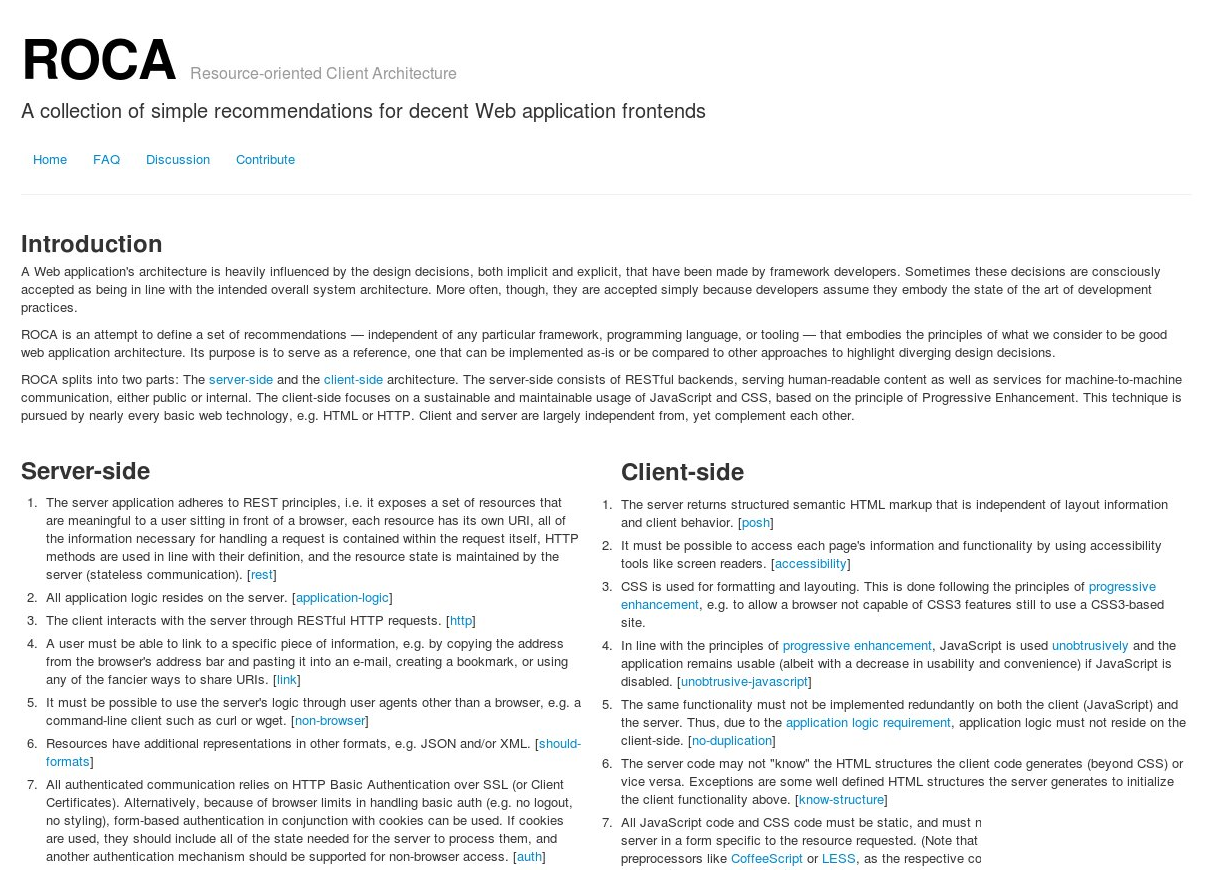
\includegraphics[width=\paperwidth]{images/roca-website.png}}
  \begin{frame}
    \vspace*{-6.4cm}
    \href{http://roca-style.org}{roca-style.org}

  %NOTE proposition for modern, maintainable web apps & the role of the
  %NOTE front-end in particular
  \end{frame}
}

\begin{frame}
  \vspace*{-1cm}
  \textcolor{gray}{
    \begin{center}
      \textbf{
        \fontsize{60}{50}\selectfont Yet another Manifesto?
      }
    \end{center}
  }

  %NOTE * innoQ: consultants - the good kind?
  %NOTE * plethora of possible approaches
  %NOTE * implicit assumptions (often due to frameworks)
  %NOTE * demand for guidance/expertise
\end{frame}

{
  \usebackgroundtemplate{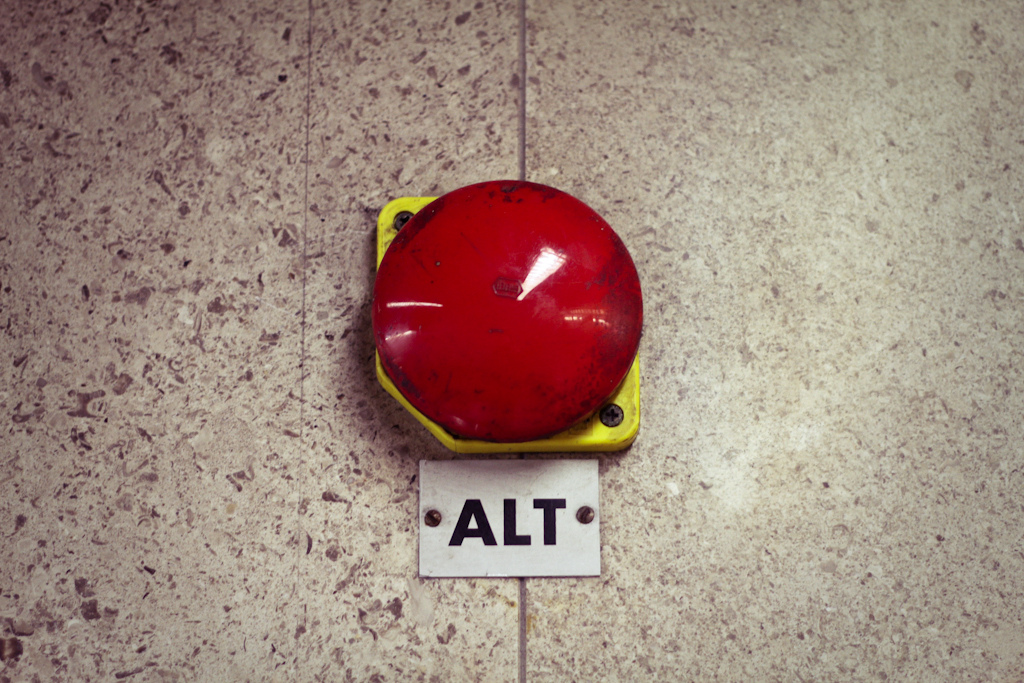
\includegraphics[width=\paperwidth]{images/buzzer.jpg}}
  \begin{frame}
    \vspace*{6.7cm}
    \tiny source: \href{http://www.flickr.com/photos/sensorsicht/5338348801/}{Hannes Fritz}

  %NOTE "label it!"
  %NOTE * makes it referenceable
  %NOTE * triggered discussion
  %NOTE * articulation makes assumptions explicit
  %NOTE
  %NOTE ROCA == set of recommendations to frame architectural discussions
  %NOTE /!\ not scripture - challenge it!
  \end{frame}
}

\subsection{MUST criteria}

\begin{frame}
  \vspace*{-1cm}
  \textcolor{gray}{
    \begin{center}
      \textbf{
        \fontsize{60}{50}\selectfont So tell us about it!
      }
    \end{center}
  }
\end{frame}

\begin{frame}{REST}
  The server application adheres to REST principles

  \begin{itemize}
    \item it exposes meaningful resources
    \item each resource has its own URI
    \item all necessary request handling information is contained within the request
    \item HTTP methods are used in line with their definition
    \item resource state is maintained by the server
  \end{itemize}
\end{frame}

\begin{frame}{Application Logic on Server}
  All essential application logic resides on the server.

  \begin{itemize}
    \item a service without business logic is a database.
  \end{itemize}
\end{frame}

\begin{frame}{Non-Browser Clients}
  The server's logic should be accessible to other user clients than a browser,

  \begin{itemize}
    \item crawler, indexer (SEO fo free, yay!)
    \item alternative user agent (curl, text browser, screen reader etc.)
    \item arbitrary unanticipated usage
  \end{itemize}
\end{frame}

\begin{frame}{HTTP}
  Client-Server interaction through RESTful HTTP requests.

  \begin{itemize}
    \item well, just like that. Period.
  \end{itemize}
\end{frame}

\begin{frame}{Links}
  A user must be able to link to a specific piece of information

  \begin{itemize}
    \item e.g. by copying the address from the browser's address bar
    \item pasting it into an e-mail or IM
    \item creating a bookmark
    \item or using any of the fancier ways to share URIs
  \end{itemize}
\end{frame}

% FND
\begin{frame}{POSH}
  The server returns structured semantic HTML markup, independent of layout information or client behavior.
  \\~\\

  
\includegraphics[width=1cm]{images/bulb.png}
  HTML offers rich, standardized semantics and data structures as well as hypermedia support.
  \\~\\

  \ensuremath{\rightarrow}
  \href{http://codeartisan.blogspot.de/2012/07/using-html-as-media-type-for-your-api.html}{Using HTML as the Media Type for your API}
  \\~\\

  NB: alternative serializations are encouraged
  \\~\\

  \tiny source: \href{http://commons.wikimedia.org/wiki/File:Bombilla_amarilla_-_yellow_Edison_lamp.svg}{Ignacio Javier Igjav}
\end{frame}

% FND
\begin{frame}{Unobtrusive JavaScript}
  JavaScript is used unobtrusively

  \begin{itemize}
    \item the application remains usable without JavaScript
    \item usability enhancements and convenience features are added progressively
  \end{itemize}
\end{frame}

\subsection{SHOULD criteria}

\begin{frame}
  \vspace*{-1cm}
  \textcolor{gray}{
    \begin{center}
      \textbf{
        \fontsize{60}{50}\selectfont Some more details, please?
      }
    \end{center}
  }
\end{frame}

\begin{frame}{Formats}
  Resources have additional representations in other formats.

  \begin{itemize}
    \item e.g. JSON and/or XML
    \item \dots or PDF- or XLSX reports (readonly)
  \end{itemize}
\end{frame}

\begin{frame}{Cookies}

  Cookies may not be used for purposes other than authentication or user tracking.

  \begin{itemize}
    \item no ``redirect back'' information
    \item no ``flash messages''
    \item If it's worth persisting, give it a proper server side resource!
  \end{itemize}
\end{frame}


\begin{frame}{Browser Controls}

  The browser controls like the back, forward and refresh buttons must work as expected.

  \begin{itemize}
    \item[back] \ensuremath{\rightarrow} user's last meaningful resource
    \item[refresh] \ensuremath{\rightarrow} no re-rendering of the login or home page
    \item mind the the POST verb!
  \end{itemize}
\end{frame}

\begin{frame}{Accessability}

  Each page's information and functionality must be accessible by tools like screen readers.

  \begin{description}
    \item[keyboard shortcuts:] fine, but not everyone uses a keyboard
    \item[pointing devices:] likewise
  \end{description}

  \ensuremath{\rightarrow} be nice to blind or otherwise handicapped people!
\end{frame}


\begin{frame}{No Duplication}

  The same functionality must not be implemented redundantly on both, client and server.

  \begin{itemize}
    \item[\ensuremath{\rightarrow}] no application logic on the client (JavaScript)
  \end{itemize}
\end{frame}

\begin{frame}{Structure Knowlegde}

  The server code may not ``know'' the HTML structures generated by client code or vice versa.

  \begin{description}
    \item[Exception:] well defined, server generated HTML to initialize client functionality
  \end{description}
\end{frame}

\begin{frame}{CSS}

  CSS is used for formatting and layouting

  \begin{itemize}
    \item following the principles of progressive enhancement
  \end{itemize}
\end{frame}

\begin{frame}{Static assets}

  All JavaScript- and CSS code must be static.

  \begin{itemize}
    \item it must not be dynamically generated for the requested resource
    \item this does not prohibit the use of preprocessors like CoffeeScript or LESS
  \end{itemize}
\end{frame}

\section{Quiz Time!}

\begin{frame}
  \vspace*{-1cm}
  \textcolor{gray}{
    \begin{center}
      \textbf{
        \fontsize{50}{50}\selectfont It's your turn.
      }
    \end{center}
  }
\end{frame}

\begin{frame}{\insertsectionhead}
  \vspace*{0.5in}

  \begin{columns}
    \begin{column}{2.2cm}
    \end{column}

    \begin{column}{2.2cm}
      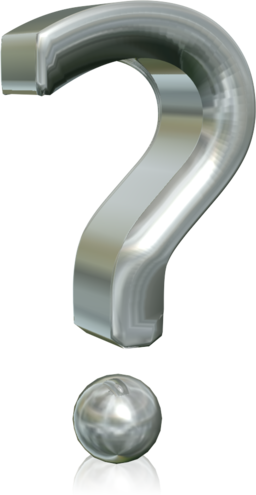
\includegraphics[width=2cm]{images/quiz.png}
    \end{column}

    \begin{column}{6.6cm}
      ROCA or not
      \vspace{0.3cm}
      \begin{itemize}
        \item[$\square$] \rocaok
        \item[$\square$] \rocafail
      \end{itemize}
    \end{column}
  \end{columns}

  \vspace*{0.4in}
  \tiny source: \href{http://commons.wikimedia.org/wiki/File:Question_mark_3d.png}{Hay Kranen}
\end{frame}

\begin{frame}
  When sharing a URL with another user, that user is presented with an empty page.

  \vspace{0.3cm}
  \begin{itemize}
    \item<1|only@1>[\Large $\square$] \Large ROCA?
    \item<2|only@2>[\Large \rocafail] \Large ROCA?
    \item<2> session state?
    \item<2> JavaScript problem?
    \item<2> hashbang URIs?
  \end{itemize}

  %NOTE e.g. due to JavaScript errors (cf. Gawker hashbang URIs)
  %NOTE e.g. due to session state
\end{frame}

\begin{frame}
  When refreshing the page, the user is taken to the respective site's front page.

  \vspace{0.3cm}
  \begin{itemize}
    \item<1|only@1>[\Large $\square$] \Large ROCA?
    \item<2|only@2>[\Large \rocafail] \Large ROCA?
    \item<2> client side logic?
    \item<2> HTML 5 history API?
    \item<2> where's the REST?
  \end{itemize}

  %NOTE URI/resource violation (e.g. bookmarks, sharing)
\end{frame}

\begin{frame}
  After using the browser's back button, the user is presented with an error
  messsage informing them to use the website's own navigation controls instead.

  \vspace{0.3cm}
  \begin{itemize}
    \item<1|only@1>[\Large $\square$] \Large ROCA?
    \item<2|only@2>[\Large \rocafail] \Large ROCA?
    \item<2> where's the REST?
  \end{itemize}

  %NOTE URI/resource violation
\end{frame}

\begin{frame}
  Shortly after starting a booking process for a train journey, the user is
  interrupted and returns several minutes later to complete his booking. Filling
  out and submitting the form, he is presented with a session timeout message.

  \vspace{0.3cm}
  \begin{itemize}
    \item<1|only@1>[\Large $\square$] \Large ROCA?
    \item<2|only@2>[\Large \rocafail] \Large ROCA?
    \item<2> Authentication \#fail?
    \item<2> Session state on server?
  \end{itemize}

  %NOTE REST stateless violation
\end{frame}

\begin{frame}
  On a slow connection, ads, navigation elements, footers and other secondary
  information are slowly displayed first. Eventually, the main content is displayed.

  \vspace{0.3cm}
  \begin{itemize}
    \item<1|only@1>[\Large $\square$] \Large ROCA?
    \item<2|only@2>[\Large ?] \Large ROCA?
    \item<2> technically OK, but annoying.
    \item<2> opinions?
  \end{itemize}

  %NOTE POSH violation? not strictly
\end{frame}

\begin{frame}
  Dashboard contents are loaded asynchronously via AJAX.

  \vspace{0.3cm}
  \begin{itemize}
    \item<1|only@1>[\Large $\square$] \Large ROCA?
    \item<2|only@2>[\Large \rocaok] \Large ROCA?
    \item<2> progressive enhancement from simple Links
  \end{itemize}

  %NOTE fine - as long as it's POSH-based
\end{frame}

\begin{frame}
  When refreshing a page displaying search results, the browser prompts the
  user to confirm whether they really want to submit the form again.

  \vspace{0.3cm}
  \begin{itemize}
    \item<1|only@1>[\Large $\square$] \Large ROCA?
    \item<2|only@2>[\Large \rocafail] \Large ROCA?
    \item<2> mind the POST verb!
  \end{itemize}

  %NOTE REST verb violation
\end{frame}

\begin{frame}
  Comments are loaded asynchronously after the page has loaded.

  \vspace{0.3cm}
  \begin{itemize}
    \item<1|only@1>[\Large $\square$] \Large ROCA?
    \item<2|only@2>[\Large \rocaok] \Large ROCA?
    \item<2> depends on implementation
    \item<2> link to comments?
  \end{itemize}

  %NOTE depends on the implementation: Disqus bad, link good
\end{frame}

\begin{frame}
  The current page's JavaScript source code is minified and obscured, thus hard
  to read.

  \vspace{0.3cm}
  \begin{itemize}
    \item<1|only@1>[\Large $\square$] \Large ROCA?
    \item<2|only@2>[\Large \rocaok] \Large ROCA?
    \item<2> technically.
  \end{itemize}

  %NOTE fine (sadly)
\end{frame}

\begin{frame}
  After clicking the ``proceeed with secure payment'' link, a browser popup window
  warns about an untrusted SSL certificate. After confirming its trust, a second
  popup asks for the user's login credentials.

  \vspace{0.3cm}
  \begin{itemize}
    \item<1|only@1>[\Large $\square$] \Large ROCA?
    \item<2|only@2>[\Large \rocaok] \Large ROCA?
    \item<2> HTTP basic auth over SSL, perfect.
    \item<2> wanna talk about trusted CAs?
  \end{itemize}

  %NOTE perfect, especially for intranet stuff. for public sites, see next slide.
\end{frame}

\begin{frame}
  Because of browser limitations in handling basic auth (e.g. no logout, no styling),
  form-based authentication in conjunction with cookies is being used.

  \vspace{0.3cm}
  \begin{itemize}
    \item<1|only@1>[\Large $\square$] \Large ROCA?
    \item<2|only@2>[\Large \rocaok] \Large ROCA?
    \item<2> OK, if all necessary state information is stored in the cookie.
    \item<2> Basic auth for non-browser clients
  \end{itemize}

  %NOTE fine, but if cookies are used, they should include all of the state needed for
  %NOTE the server to process them, and another authentication mechanism should be
  %NOTE supported for non-browser access
\end{frame}


\begin{frame}
  Inpecting the current page's source code reveals a minimal HTML frame with
  JSON data embedded in a \texttt{<SCRIPT>} tag.

  \vspace{0.3cm}
  \begin{itemize}
    \item<1|only@1>[\Large $\square$] \Large ROCA?
    \item<2|only@2>[\Large \rocafail] \Large ROCA?
    \item<2> think POSH!
    \item<2> think PE!
  \end{itemize}

  %NOTE JavaScript dependency violation (cf. Google Plus)
\end{frame}

\begin{frame}[fragile]
  Selecting ``open link in new tab'' results in a blank page.

  \vspace{0.3cm}
  \begin{itemize}
    \item<1|only@1>[\Large $\square$] \Large ROCA?
    \item<2|only@2>[\Large \rocafail] \Large ROCA?
    \item<2> bad: \mint{html}|<a href="javascript:">|
    \item<2> different, yet still bad: \mint{html}|<a href="#">|
  \end{itemize}

  %NOTE e.g. due to <a href="javascript:;">
  %NOTE different, but still invalid: <a href="#">
\end{frame}

\begin{frame}
  Form inputs from a previous step are stored in Cookies to be retrieved by
  JavaScript for validations in the next step.

  \vspace{0.3cm}
  \begin{itemize}
    \item<1|only@1>[\Large $\square$] \Large ROCA?
    \item<2->[\Large \rocafail] \Large ROCA?
    \item<2-> Session state?
    \item<2-> Application logic on Client?
    \item<3> think of a better solution?
  \end{itemize}

  %NOTE e.g. a multi-step wizard.
\end{frame}

\begin{frame}
  TODO: redirect session data, multi-tab conflicts
  e.g. stilkov: "Creating a second window does not create an independent view, but confuses the application's control flow concept"

  \vspace{0.3cm}
  \begin{itemize}
    \item[$\square$] \ding{51}
    \item[$\square$] \ding{55}
  \end{itemize}

  %NOTE TODO
\end{frame}

\begin{frame}
  \vspace*{-2cm}
  \textcolor{gray}{
    \begin{center}
      \textbf{ \fontsize{50}{80} \selectfont You did well. \\ }
      {\fontsize{30}{30} \selectfont Thank you!}
    \end{center}
  }
\end{frame}


\begin{frame}{Contact}
  \begin{columns}
    \column{5cm}
    
\includegraphics[width=4cm]{images/innoQ-Logo-RGB-72dpi.png}
    \vspace{4mm}
    \column{4.5cm}

    \href{http://www.innoq.com}{http://www.innoq.com} \\
    \href{mailto:info@innoq.com}{info@innoq.com}
  \end{columns}

  innoQ Deutschland GmbH \\
  Krischerstraße 100 \\
  D-40789 Monheim \\
  Tel (+49) 2173 3366 0
\end{frame}

\end{document}
